%% LyX 2.1.4 created this file.  For more info, see http://www.lyx.org/.
%% Do not edit unless you really know what you are doing.
\documentclass[12pt,english]{article}
\usepackage[T1]{fontenc}
\usepackage[latin9]{inputenc}
\usepackage{amsmath}
\usepackage{graphicx}

\makeatletter

%%%%%%%%%%%%%%%%%%%%%%%%%%%%%% LyX specific LaTeX commands.
%% Because html converters don't know tabularnewline
\providecommand{\tabularnewline}{\\}

%%%%%%%%%%%%%%%%%%%%%%%%%%%%%% User specified LaTeX commands.
\usepackage{tikz}
\usetikzlibrary{calc}

\makeatother

\usepackage{babel}
\begin{document}

\title{Reading on Directed Search}


\author{Michael Peters}

\maketitle
This reading will describe a model that is used extensively in macroeconomics
to understand labor markets. The model is a part of a larger literature
on search and matching. I'll explain the model in its simplest form
here. Richer variants of the model can be used to understand wage
distributions and unemployment duration. The model has also been used
to do econometric evaluation of labor markets.


\section{Bertrand Equilibrium}

The model of directed search emerged as a response to something called
\emph{Bertrand Equilibrium }- a model designed to understand price
competition. So I'll describe it first. In the Bertrand model, there
are two firms. They have constant production costs, say $c_{1}$ for
firm 1 and $c_{2}<c_{1}$for firm 2. There is a consumer who has some
utility function $u\left(q,P\right)$ describing her payoff when she
buys $q$ units in total and pays price $P$ for them. We want to
assume $u$ is increasing in $q$ and decreasing in $P$. We'll assume
that $u\left(Q\left(p\right),pQ\left(p\right)\right)\ge u\left(q,pq\right)$
for all $q$. In other words, the consumer's demand curve is $Q\left(p\right)$.
Of course, the consumer can allocate her purchases between the two
firms in any way that she wants - lets just use $q_{1}$ to be the
amount she buys from firm 1 and $q_{2}$ as the amount she buys from
firm 2.

As we will use this below, let $p_{i}^{\ast}$ be the \emph{monopoly
price }for firm $i$\emph{$,$ }i.e, it is the price that maximizes
$pQ\left(p\right)-c_{i}Q\left(p\right)$

To describe the game we need to describe the strategies of each of
the three players and the payoffs that are associated with each set
of strategies. For strategies, firms just set prices. The consumer
must choose how much to buy from each firm for each pair of prices
that the firms choose. Payoffs for firm 1
\[
\pi_{1}\left(p_{1},p_{2},q_{1}\left(\cdot\right),q_{2}\left(\cdot\right)\right)=p_{1}q_{1}\left(p_{1},p_{2}\right)-c_{1}q_{1}\left(p_{1},p_{2}\right)
\]
and for firm 2
\[
\pi_{2}\left(p_{1},p_{2},q_{1}\left(\cdot\right),q_{2}\left(\cdot\right)\right)=p_{2}q_{2}\left(p_{1},p_{2}\right)-c_{2}q_{2}\left(p_{1},p_{2}\right).
\]
For the consumer payoffs are $U\left(q_{1}+q_{2},p_{1}q_{1}+p_{2}q_{2}\right)$.

Lets use subgame perfect Nash equilibrium as our solution concept.
Then we can use backward induction to figure out what everyone will
do. Even using backward induction, to describe an equilibrium what
we need to do is to specify the strategies that each of the players
are using. For firms this is easy, just prices. For consumers it is
more complicated.

We have to write down what the consumer is expected to do in response
to any pair of prices she faces. Recall that the reason we have to
do this is because the firms calculated their best price offer by
considering what they would get by deviating to other offers. Subgame
perfection requires the firms to believe that when they deviate, the
consumer will respond in a sensible way. What that means in this context
is that firms should believe that consumers will respond by buying
only at the lowest price. When firms offer the same price, it doesn't
matter which firm the consumer buys from. Nevertheless, to specify
a strategy we have to specify exactly what consumers will do when
prices are equal. We write this down formally as follows:
\begin{eqnarray}
q_{1}\left(p_{1},p_{2}\right) & = & \begin{cases}
Q\left(p_{1}\right) & p_{1}<p_{2}\\
0 & \mbox{otherwise.}
\end{cases}\label{consumer1}
\end{eqnarray}
For firm 2, the corresponding strategy is
\begin{equation}
q_{2}\left(p_{1},p_{2}\right)=\begin{cases}
Q\left(p_{2}\right) & p_{2}\le p_{1}\\
0 & \mbox{otherwise.}
\end{cases}\label{consumer1-1}
\end{equation}


This relatively simple pair of expressions hides a very important
restriction. The strategy specified above has the property that the
consumer will buy everything from firm 2 as long as firm 2's price
is \emph{less than or equal }to firm 1's price. There are a continuum
of other strategies we could have used, all of which would have specified
different actions when the firms set the same price. Later you will
see why the strategy specified above is the only one that supports
a subgame perfect equilibrium.

Given the strategy specified above for consumers, we now want the
firms to choose prices that are best replies. Start with firm 1 and
suppose he is facing a price for firm 2 equal to $p_{2}$. There are
two easy cases. If $p_{2}>p_{1}^{\ast}$, then it should be apparent
that firm $1$ will want to respond by setting price equal to $p_{1}^{\ast}$.
This has to be better than setting any price at or above firm 2's
price, since 1 either won't get any demand at such a price, or will
sell some amount that earns him less profit than he could get by charging
what he would as a monopolist. Alternatively, if firm 2 has a price
below $c_{1}$, then firm 1 can set any price that is no smaller than
firm 2's price. This will ensure that he doesn't have to sell output
at a price less than his marginal cost because of the way we specified
the consumer's strategy in (\ref{consumer1}) and (\ref{consumer1-1})
above.

The funny stuff starts when firm 2 charges a price that is between
$p_{1}^{\ast}$ and $c_{1}$. If that is the case, then firm 1 can
sell some quantity at prices above his marginal cost and make a profit.
In that case he won't want to set a price at or above $p_{2}$, for
then he will get nothing. He needs to set a price below $p_{2}$ in
order to make profitable sales. Since $p_{2}$ is below his monopoly
price, he also wants to set his price as close to $p_{1}$ as possible.
No matter what price below $p_{2}$ he sets, he can always get the
price a little closer. In other words, firm 1 \emph{doesn't have a
best reply. }

This may seem a little confusing. Yet it is actually somewhat helpful.
It means that we are never going to be able to find a subgame perfect
equilibrium where firm 2 sets a price above $c_{1}$. Why? Well, a
subgame perfect equilibrium is a Nash equilibrium, so both firms need
to set prices that are best replies. Since we can never find a best
reply for firm 1, we can rule out such an outcome.

Once firm 2's price falls to $c_{1}$, firm 1 has a lot of best replies
- any price at or above firm 2's price will ensure that 1 doesn't
make any sales. This is true even if firm 1 matches firm 2's price
because of the way we specified the consumer's strategy in (\ref{consumer1})
and (\ref{consumer1-1}). 

The outcome that is usually referred to as 'the' equilibrium in the
Bertrand game is the one where both firms set the price and the consumer
uses the strategy described by (\ref{consumer1}) and (\ref{consumer1-1})
above.

To understand why this is a Nash equilibrium you need to check unilateral
deviations. First of all, you already know that the consumer's strategy
is a best reply to the prices set by firms, because this strategy
has the consumer doing her best no matter what the firms do. Firm
2 sets the price $c_{1}$ and sells $Q\left(c_{1}\right)$ units at
a price which is strictly above his marginal cost. So he makes a profit.
If he raises price, he loses all his profitable sales. So raising
price is not a profitable deviation. If he lowers price he sells a
bit more at a lower price. Since $c_{1}$ must also be below firm
2's monopoly price, this isn't profitable.

Firm 1 sells nothing in this equilibrium. If he raises price, he still
sells nothing. If he lowers price, he will make sales, but at a price
that is below his marginal cost. So firm 1 has no profitable deviation.

There are a bunch of other equilibrium outcomes like this one. Can
you see why the same arguments can be used to support subgame perfect
equilibrium with both firms charging any price between $c_{1}$ and
$c_{2}$? Given the way we have specified the consumer's strategy,
we can support any such price by having firm1 match firm 2's price.
This keeps firm 2 from wanting to raise its price. Firm 1 is happy
with this because he doesn't make any sales in equilibrium.


\subsection{Problems to Think About}
\begin{enumerate}
\item We could change the strategy that the consumer is using in a subgame
perfect equilibrium by having her buy half of her demand from each
firm when the two firms set the same price. Can you explain why it
is impossible to construct a Subgame perfect equilibrium in which
the consumer uses this strategy?
\item Explain why there is a continuum of Nash equilibrium outcomes for
this game in which firms set any common price between $c_{1}$ and
$p_{1}^{\ast}$, while the consumer buys half her demand from each
firm when prices are the same.
\end{enumerate}

\section{Directed Search}

Though Bertrand equilibrium is useful in explaining how subgame perfection
works in games where players have a continuum of strategies, it describes
an equilibrium that just doesn't seem plausible. For example, both
firms set the same price even though they have different costs. For
most products there is a lot of price variability between firms that
doesn't seem to be related to difference in product quality (Apple
computers versus everything else for example - or Microsoft Office
versus OpenOffice).

Directed search is one of the models that has been proposed to deal
with this. It has some very useful characteristics, especially when
applied to labor markets, where it can be used to explain unemployment.
The search decisions that workers make in a directed search model
lead to unemployment and unfilled vacancies even though workers can
see all the firms' wages when they make their search decisions. The
reason it is called directed search is that workers decisions about
where to apply are guided or directed by wages. This distinguishes
the model from a much bigger literature that assumes that workers
and firms are matched randomly (by chance).

To see how it works, suppose that as in the story above, there are
two firms. Instead of setting prices, though, they set wages. Each
of the firms want to fill exactly one vacancy. Instead of a single
consumer, we'll assume there are two workers who try to find jobs
with these two firms. The way directed search approaches this is to
assume that each of the workers makes an application to one and only
one of the firms. Each of the firms then collects its applications
and hires one of the workers who applied. If two workers apply to
the same firm, the firm chooses one of them randomly and offers her
the job. If only one worker applies, the firm just offers the job
to that worker. 

To keep the story simple, we will assume that firms who get no applications
are just out of luck, as are workers who apply but aren't offered
a job. Otherwise, we'll assume that firm 1 earns gross profit $y_{1}$
if it fills its vacancy, while firm 2 earns $y_{2}<y_{1}$. Workers'
payoffs are just the wages they earn.

What gives the directed search model nice properties is the assumption
that workers use a \emph{symmetric }application strategy. What that
means is that each of the workers applies to firm 1 with the same
probability $\pi$. This is something you are familiar with - a mixed
strategy equilibrium. The extra part here is that firms will have
to figure out how changes in their wages are going to affect the mixed
strategy equilibrium for the workers' application game. Since workers'
mixed strategies are going to mean that some worker don't get jobs,
there is going to be some unemployment and some unfilled vacancies.
Firms can limit the probability with which they have unfilled vacancies
by raising wages, since that will increase the probability with which
workers apply. We'll work out the wages that firms offer in a subgame
perfect equilibrium. The outcome won't look anything like the equilibrium
of the Bertrand pricing game that we studied above.

Lets do backward induction and try to figure out what the workers
will do for every pair of offers by the firms. Call the wages of the
two firms $w_{1}$ and $w_{2}$ for firm 1 and 2 respectively. Strictly
speaking, we should model what the firms do once they receive applications,
but will skip that for brevity and just assume as above that the firms
mechanically select each worker with probability $\frac{1}{2}$ when
it has two applications.

The normal form of the application game played among the workers now
looks like the following:

\begin{center}
\begin{tabular}{|c|c|c|}
\hline 
 & Firm 1 & Firm 2\tabularnewline
\hline 
\hline 
Firm 1 & $\frac{w_{1}}{2}$,$\frac{w_{1}}{2}$ & $w_{1},w_{2}$\tabularnewline
\hline 
Firm 2 & $w_{2},w_{1}$ & $\frac{w_{2}}{2}$,$\frac{w_{2}}{2}$\tabularnewline
\hline 
\end{tabular}
\par\end{center}

To understand the payoffs, just observe that if both workers apply
to the same firm, they each get the job with probability $\frac{1}{2}$.
That makes an expected payoff equal to $\frac{w_{1}}{2}$ for both
of them when they both apply to firm 1.

If the other worker is applying to firm 1 with probability $\pi$,
then the expected payoff to the worker if he applies there is
\[
\pi\frac{w_{1}}{2}+\left(1-\pi\right)w_{1}.
\]
The explanation is that if the other worker also applies to firm 1,
then there is half a chance that the worker will be hired. If the
other worker applies to firm 2, then the worker is hired for sure.

Using the same reasoning to compute the expected payoff associated
with an application to firm 2, the probability with which the worker
expects the other worker to apply to firm 1 had better satisfy
\begin{equation}
\pi\frac{w_{1}}{2}+\left(1-\pi\right)w_{1}=\pi w_{2}+\left(1-\pi\right)\frac{w_{2}}{2}\label{equality}
\end{equation}
or 
\[
\pi=\frac{2w_{1}-w_{2}}{w_{1}+w_{2}}.
\]


Now you should recognize that in order to describe a subgame perfect
equilibrium, you need to specify how workers will react to \emph{all
}pairs of wages, not just to those you think are important. In the
expression above some weird stuff can happen when wages get too far
apart. First, if $w_{2}>2w_{1}$, the solution to the equation above
is negative, so something is wrong. In this case, think ``one of
the actions has become dominated''. If you look back at the payoff
matrix you can see which one - $w_{2}$ is so high that the worker
would rather go to firm 2 than firm 1 even if he were sure that the
other worker were going to apply to firm 2.

Another way to look at it is that in order to satisfy (\ref{equality})
it isn't enough just to maximize the probability with which the other
worker applies at the same firm, you have to go even further and change
the weight assigned to the good outcome so that the payoff turns negative.

Exactly the same thing occurs when $w_{1}>2w_{2}$ (so that the solution
to (\ref{equality}) is greater than 1). Then applying at firm 2 is
a dominated strategy.

What this algebra tells us is that the only symmetric subgame perfect
equilibrium strategy looks like this:
\begin{equation}
\pi\left(w_{1},w_{2}\right)=\begin{cases}
\frac{2w_{1}-w_{2}}{w_{1}+w_{2}} & \frac{w_{1}}{2}\le w_{2}\le2w_{1}\\
1 & w_{2}<\frac{w_{1}}{2}\\
0 & \mbox{otherwise.}
\end{cases}\label{strategy}
\end{equation}


This last formula says that firm 1 should expect that varying its
wage will change the probability with a worker applies in the Nash
equilibrium of the workers' application game. How exactly? Well, you
can read this from the formula - using the quotient rule
\[
\frac{d\pi\left(w_{1},w_{2}\right)}{dw_{1}}=
\]
\begin{equation}
\frac{d}{dw_{1}}\frac{2w_{1}-w_{2}}{w_{1}+w_{2}}=\frac{\left(w_{1}+w_{2}\right)2-\left(2w_{1}-w_{2}\right)}{\left(w_{1}+w_{2}\right)^{2}}=\frac{3w_{2}}{\left(w_{1}+w_{2}\right)^{2}}>0\label{derivative}
\end{equation}
provided $\frac{w_{1}}{2}\le w_{2}\le2w_{1}$. Otherwise this derivative
is zero.

If you write down what firm 1's expected profit is you get
\[
\left(1-\left(1-\pi\right)^{2}\right)\left(y_{1}-w_{1}\right).
\]
The logic is that firm 1 is going to fill its vacancy provided at
least one of the workers applies. The probability that neither of
them applies is $\left(1-\pi\right)^{2}$ - which gives the formula. 

At this stage, lets make a guess about what equilibrium is going to
look like. First, notice that there is no point for firm 1 to offer
a wage more than twice $w_{2}$ or less than half $w_{2}.$ In the
first case, he would get applications from both workers for sure,
and would still get these applications if he cut his wage a bit. In
the latter case, he wouldn't get any applications at all, so he wouldn't
make any profit. This means that in any subgame perfect equilibrium,
the wages of the firms are going to be close enough together that
the application probability will be determined by the solution to
(\ref{equality}). Given this, it isn't too hard to see how firm 1
would choose its wage? Maximize the firm's profit by choosing the
wage that makes the derivative of this profit function 0. That is,
find $w_{1}$ by solving the equation
\begin{equation}
2\left(y_{1}-w_{1}\right)\frac{d\pi}{dw_{1}}\left(1-\pi\right)=\left(1-\left(1-\pi\right)^{2}\right)\label{first-order-condition}
\end{equation}
 where $\pi$ is given by (\ref{strategy}) and $\frac{d\pi}{dw_{1}}$
is given by (\ref{derivative}). The solution to this equation gives
the best reply function for firm 1.

At this point, even the computer algebra programs are going to fail
to find solutions for you, though you could try for numerical solutions.
The literature on directed search has handled this by developing models
with a continuum of workers and firms and using these to approximate
large labor markets. Instead of studying those, lets just look at
a special case that is analytically tractable (though a little too
special to be of much practical use). If the profits the firms make
are the same (lets say $y_{1}=y_{2}=y$), then it seems plausible
that both firms would set the same wage in a subgame perfect equilibrium.
If they did, the probability with which each worker would apply to
them would be $\frac{1}{2}$. Whatever common wage they set should
satisfy the first order condition (\ref{first-order-condition}) for
both firms. This first order condition would then simplify to 
\[
2\left(y_{1}-w_{1}\right)\frac{1}{2}\frac{3}{4w}=\frac{3}{4}
\]
This has a very simple solution $w=\frac{y}{2}$. 

What this means is that there is only one wage, $\frac{y}{2}$ that
could satisfy the first order condition that is required to hold when
firms wages are best replies to one another. This means either that
the wages both firms offer in the subgame perfect equilibrium are
equal to $\frac{y}{2}$, or that there is no pure strategy equilibrium
at all. There are some second order conditions that need to hold.
Lets leave those for some future headache and just take it for granted
that the subgame perfect equilibrium has both firms offering the wage
$\frac{y}{2}$ while the workers both use the strategy described in
(\ref{strategy}). 

The equilibrium in which the firms are identical and set the same
wage isn't completely satisfactory. It hides one of the main predictions
of directed search, i.e., it is harder to get a job at a higher wage.
Of course, everyone knows that it is harder to get a job at a high
wage firm. The advantage of the model is that you now have a precise
explanation of what 'harder to get a job' means. This makes it possible
to turn our intuition into formal predictions that we can check by
looking at data.


\subsection*{Problems:}
\begin{enumerate}
\item Find the application probability $\pi$ to be used by both workers
that maximizes the expected number of matches (which is the same as
the expected level of employment). Do you see any connection with
the Price of Anarchy theorem?
\item Find the application probability $\pi$ to be used by both workers
that maximizes expected revenues of firms.
\item Assuming that all firms offer the same wage, write out the Nash equilibrium
application probabilities for workers when there are three firms and
two workers.
\end{enumerate}

\subsection{How a model evolves}

The model I showed you above is pretty restrictive. Firms are the
same, workers are the same. Workers don't care where they work, the
just care about the wage they get, and so on. Many models in economics
are like this - just rich enough to illustrate the basic principles,
and to turn intuition into prediction, but not really rich enough
to explain what we see going on in a real labor market.

If we just take the basic prediction of the model - it will take workers
longer to find jobs at higher wage firms - then we will probably be
confused by some of the things we will see in real markets - they
just won't behave exactly the way we want them to. One response would
be to give up and abandon the model when it doesn't work. A more useful
approach is to let the model itself suggest the changes you need to
make to understand your data.

Since this is such a common life story for models in economics, it
might pay just to diverge a bit so I can illustrate how this might
work. Some of my colleagues, Pai Xu, from the University of Hong Kong,
and Kun Li from the Toulouse School of economics, have assembled a
dataset of executive compensation collected from Compustat (which
you can look up on wikipedia) that contains observed characteristics
of both executives and the firms for which they worked, for a period
from 1993 to 2009. This data contains observations on executives'
age, their gender, the firms for which they worked and their total
wages and bonuses for each of the years in which these executive appeared
in the sample. For the firms, the database contains information of
total assets (AT), sales, employment size (EMP), income before extraordinary
(OIBDP), standard industry classification code (SIC). 

The nature of the data is such that an individual can be observed
over a number of different years. You can see the compensation that
he or she received each year, as well as how many years he or she
remained in each job. The duration of the sample, 1993 to 2009 means
there are a lot of observations. The regression I'll show you has
over 10,000 observations of job transitions (movements from one job
to another) for the executives in the sample. I'll just just show
you how information from data like this would be used to refine our
thinking about the model

Here is a summary that describes a bit what the data looks like.

\begin{center}
\includegraphics[scale=0.6]{/home/peters/files/docs/matching_by_luck/mike/Tc}
\par\end{center}

It isn't apparent from this table, but the first somewhat problematic
observation suggested by this data is that there doesn't appear to
be much unemployment. Directed search is about unemployment, about
how workers made applications, and about how they are eventually matched
with firms. At least as the information appears in this dataset, the
executives never appear to be unemployed. They seem to move from one
job directly into another, either internally (for example, in the
table, in 1993, 521 of the executives moved to higher paying jobs
within the firm that already employed them), or by moving between
jobs. There were short spells of unemployment for some of the executives,
but they happened within a year and were too short for most part to
register in the yearly data. What to do about this? Well, the workers
moved, so they must have been searching on the job. 

The advantage of all the work we did on the basic model, is that we
can now see that it would't really be too hard to incorporate this.
As we described the model above, if two worker apply for the same
job, one of them is unlucky and gets nothing. We coudl as easily assume
that the unlucky worker just returns to his old job instead. Since
our first version gave us a probability with which each worker would
get a job, we could just add this 'on the job search' and calculate
moving probabilities (and success probabilites) for workers who are
currently employed at different wages. That will give us something
we can look for in our data. 

Return to the payoff matrix that we used to describe the problem faced
by unemployed workers. Lets just modify it by assuming that if both
workers applied at the same firm, then the one who does not get the
job just goes back to his old job. Suppose worker 1 is working at
wage $w_{0}^{1}$ while worker 2 is working at wage $w_{0}^{2}$.
There is a pair of vacancies offering wages $w_{1}$ and $w_{2}$
with $w_{2}>w_{1}$. Since we are just trying to get going at this
point, lets assume that both $w_{1}$ and $w_{2}$ are larger than
$w_{0}^{1}$ and $w_{0}^{2}$. Then the payoff matrix looks like this

\begin{center}
\begin{tabular}{|c|c|c|}
\hline 
 & $w_{1}$ & $w_{2}$\tabularnewline
\hline 
\hline 
$w_{1}$ & $\frac{1}{2}w_{1}+\frac{1}{2}w_{0}^{1}$,$\frac{1}{2}w_{1}+\frac{1}{2}w_{0}^{2}$ & $w_{1},w_{2}$\tabularnewline
\hline 
$w_{2}$ & $w_{2},w_{1}$ & $\frac{1}{2}w_{2}+\frac{1}{2}w_{0}^{1}$,$\frac{1}{2}w_{2}+\frac{1}{2}w_{0}^{2}$\tabularnewline
\hline 
\end{tabular}
\par\end{center}

The symmetric equilibrium requires that worker 2 apply with firm 1
with probability $\pi_{2}$ such that
\[
\pi_{2}\left(\frac{1}{2}w_{1}+\frac{1}{2}w_{0}^{1}\right)+\left(1-\pi_{2}\right)w_{1}=\pi_{2}w_{2}+\left(1-\pi_{2}\right)\left(\frac{1}{2}w_{2}+\frac{1}{2}w_{0}^{1}\right).
\]
 That is 
\[
\pi_{2}=\frac{w_{0}^{1}+w_{2}-2w_{1}}{2w_{0}^{1}-w_{2}-w_{1}}.
\]
Of course, we need to check for situations in which this is negative
or greater than 1. At this point, we are just trying to get some idea
about how on the job search works, so as a first approximation, lets
assume that $w_{1}$ and $w_{2}$ are close together, and that both
of them are considerably bigger than $w_{0}^{1}$. Then (by differentiation
for example) you could see that $\pi_{2}$ is an increasing function
of $w_{1}$. 

One unusual thing about this is that the probability with which worker
2 applies to firm 1 depends on the wage at which worker 1 is currently
employed (but not on the wage at which worker 2 is currently employed).
Of course, you understand that the reason for that is that worker
2 is trying to make worker 1 indifferent. However, if you put it another
way it sounds very strange. The probability that worker 2 applies
to different firms doesn't depend directly on the wage at which he
is currently employed. This is extremely confusing, mostly because
we want to know what this is going to look like in our executive data.
We should be able to see which executives are employed at low wage
firms, which ones are employed at high wage firms. We will also see
them moving to new jobs and the wages that they get at these new jobs.
It would be nice to know whether worker who are employed at low wages
are more likely to change jobs - that seems plausible. If they do
change jobs, where will they end up going? Will they move to the highest
wage firm paying $w_{2}$, or will they be willing to settle on $w_{1}$
- a wage that is higher that the one they are currently getting, but
not the highest one available.

Its a bit tough to guess. This is why it is nice to have a model -
we can actually do the calculation and make a prediction. We have
$w_{2}>w_{1}>w_{0}^{1}>w_{0}^{2}.$ The good job is with firm 2 which
pays the higher wage. Worker 1 already has a pretty good job. While
worker 2 has a low paying job. What is the probability that worker
2 gets the good job? It is the probability he applies to firm 2, times
the probability that either worker 1 doesn't apply, or worker 1 does
apply, but firm 2 gives him the job anyway. Formally
\[
\Pr\left\{ 2\mbox{ gets the good job}\right\} =
\]
\[
\left(1-\pi_{2}\right)\left(\left(1-\pi_{1}\right)/2+\pi_{1}\right)=
\]
\[
\frac{w_{0}^{1}-2w_{2}+w_{1}}{2w_{0}^{1}-w_{2}-w_{1}}\left(\frac{w_{0}^{2}-2w_{2}+w_{1}}{2\left(2w_{0}^{2}-w_{2}-w_{1}\right)}+\frac{w_{0}^{2}+w_{2}-2w_{1}}{2w_{0}^{2}-w_{2}-w_{1}}\right)=
\]
\[
\frac{w_{0}^{1}-2w_{2}+w_{1}}{2w_{0}^{1}-w_{2}-w_{1}}\left(\frac{3w_{0}^{2}-3w_{1}}{2\left(2w_{0}^{2}-w_{2}-w_{1}\right)}\right).
\]
The probability that 1 gets the good job is derived in a similar way,
except that $w_{0}^{1}$ and $w_{0}^{2}$ are interchanged. That is
\[
\Pr\left\{ 1\mbox{ gets the good job}\right\} =
\]
\[
\frac{w_{0}^{2}-2w_{2}+w_{1}}{2w_{0}^{2}-w_{2}-w_{1}}\left(\frac{3w_{0}^{1}-3w_{1}}{2\left(2w_{0}^{1}-w_{2}-w_{1}\right)}\right).
\]
Actually it is really easy to make the comparison between these two
numbers, because most of the terms are common. All we have to do is
to compare the very first terms $w_{0}^{1}-2w_{2}+w_{1}$ and $w_{0}^{2}-2w_{2}+w_{1}.$
Since $w_{0}^{1}$ is larger than $w_{0}^{2}$, the first term is
larger, which means that the worker who is currently in the low wage
job is more likely to move up to the high wage firm than the worker
in the high wage job.

Before we move to the executive data, lets do one more calculation
(it isn't too complicated). Instead of asking who is more likely to
move to the high wage job, lets just ask who is more likely to move.
Lets start with player 2, who is currently in the low wage job. He
moves if he applies to firm 1 and gets the job, or if he applies to
firm 2 and gets the job. The formula is
\[
\Pr\left\{ 2\mbox{ moves}\right\} =
\]
\[
\left(1-\pi_{2}\right)\left(\left(1-\pi_{1}\right)/2+\pi_{1}\right)+\pi_{2}\left(\pi_{1}/2+\left(1-\pi_{1}\right)\right).
\]
If you simplify this you will get
\[
\frac{1+\pi_{1}+\pi_{2}-2\pi_{1}\pi_{2}}{2}.
\]
If you do this calculation for player 1 by interchanging the positions
of $\pi_{1}$ and $\pi_{2}$, you are going to get exactly the same
expression. In other words, the probability of moving in any period
is independent of the wage a worker is currently making. This is somewhat
surprising, but it is a prediction that we can take to our executive
data to see whether it is true in this executive labor market.

So what does the executive data say? What do I know, I am a theorist,
but I can tell you what my co-author found. Start with the first prediction
- the worker who is currently employed at the low wage is more likely
to move to the high wage firm than the worker who is currently employed
at the high wage firm. Roughly what that means is that the wages you
earn for the rest of your life should be more variable if you are
currently employed at a low wage firm, than if you are at a high wage
firm. Here is what he found for the executive data.

\begin{center}
\includegraphics[scale=0.5]{/home/peters/files/docs/matching_by_luck/mike/F2}
\par\end{center}

The 'quintiles' referred to along the bottom axis represent the collection
of executives with different wages. The quintile 1 consists of the
20\% of all the executives who had the lowest wages, quintile 5 consists
of the top 20\%. What he did was to take all the executives in 1993
who were in a quintile, then wrote down the wages of any jobs that
they moved to in the future. These were almost always (but not exclusively)
higher wages. Then he computed the standard deviation of all those
wages and plotted it as a green bar in the figure. Notice that, as
we suggested above, the standard deviation seems to be getting smaller
as you move to higher quintiles. The dashed lines represent the wage
extremes - again the range seems to be getting slightly smaller as
you move up to higher quintiles.

What about the prediction that the probability of moving to the new
job is independent of the wage. The table that follows shows what
he found:

\begin{center}
\includegraphics[scale=0.5]{/home/peters/files/docs/matching_by_luck/mike/T1}
\par\end{center}

To understand what he found, look at the two columns on the right
of this picture. They represent the result of running a regression
in which each observation has an executive working at a certain wage,
then an observation about whether or not he moved to a new job in
the future. The dependent variable (the one that we are trying to
explain) is the variable that indicates whether or not he or she moved.
The independent variable (the thing we think does the explaining)
is plnwage, the wage at which he or she is currently working. The
signs of the numbers down the column indicate whether the independent
variable caused the dependent variable to go up or down. So the .15
in the second row, third column indicates that increasing the wage
at which an executive is employed increases the probability with which
he moves. Since plnwage is the log of the wage, the way to interpret
this is that increasing the past wage by 1\% causes the probability
with which the executive moves in future to rise by .15\%. This isn't
really consistent with what our theory says.

In fact, this same table has something that is even more troubling.
The leftward two columns show the result of regressing the log of
the wage that an executive receives when he or she moves to a new
job on the time the executive spent in his or her last job. Our theory
says that since it is harder to find high wages, workers who get them
should have spent a longer time trying. The numbers associated with
duration are negative. What that means is that the longer an executive
spent in his or her last job, the lower the wage she got in her new
one.

I am explaining all this just to show what happens to a model as it
is used to examine actual data. The executive data isn't ideally suited
to the theory, since we don't see the unemployment spells. It could
be that if we had a comparable sample of factory workers, that we
might see something that looks more like what we want. Maybe it wouldn't.
Even within this data, the regressions may well be hiding confounding
factors. For example, workers who have spent a long time at their
last job are likely to be older and less attractive to prospective
employers just because they are closer to retirement. The reason they
get lower wages from longer periods of search isn't because our theory
is wrong, but because the wage is being depressed by something that
is correlated with length of employment, i.e., age. Pai tried to control
for this by adding age to the regression, but it didn't make much
difference. The point is that there may be something comparable confounding
this result. Whether we find the data is consistent with our theory
or not, we need to reserve judgment.

Even if we want to accept the fact that our model isn't really adequate
to explain the data we have, we don't just give it up. We'll make
further modifications, the same way we modified our initial model
by adding on the job search. This data set is actually suggesting
the ways we should proceed.


\subsection*{Problems:}
\begin{enumerate}
\item Work out the (symmetric) Nash equilibrium for the case where $w_{1}>w_{1}^{0}>w_{2}>w_{2}^{0}$.
\item Suppose that $w_{1}=w_{2}>w_{1}^{0}=w_{2}^{0}$, and that all firms
have the same revenue. Can you figure out how to check whether one
of the firms who currently have workers (that is, the firms that are
already employing the workers) have any incentive to raise wages to
try to prevent their workers from leaving?
\end{enumerate}

\section{Another Approach}

When two workers apply to the same firm in the story above, one of
them is chosen randomly and given the job. The unlucky worker presumably
goes back to the market and tries again with another firm. This has
a couple of implications that don't seem very plausible. First, the
wage that a worker receives doesn't say much about the worker. If
there were a distribution of wages available, then the workers who
get jobs at the high wage firms are just lucky. As a result, their
wages shouldn't be correlated at they move between jobs. Second, since
workers just repeat their application behavior in each period that
they are unemployed, the probability that they will get a job in any
period shouldn't depend on the length of time they are unemployed.
Neither of these predictions is right.

To deal with this an alternative model assumes that workers have different
types that the firm can see when they apply and the firm interviews
them. When two workers apply at the same firm, the firm just hires
the best one.\footnote{This is the two type version of the model in \cite{pet10-2}.}
A lottery is used to pick a worker only when they have the same type.
What makes the model run is that workers don't know how good or bad
their competitors are.

To see how this one works, let the types be $h$ and $l$. Suppose
that the types of the two workers are independently drawn, and that
each worker is believed to have type $h$ with probability $\lambda$.
The payoff matrix faced by a worker then depends on his or her type.
The matrix for a type $h$ worker looks like this

\begin{center}
\begin{tabular}{|c|c|c|}
\hline 
 & Firm 1 & Firm 2\tabularnewline
\hline 
\hline 
Firm 1 & $\lambda\frac{w_{1}}{2}+\left(1-\lambda\right)w_{1}$ & $w_{1}$\tabularnewline
\hline 
Firm 2 & $w_{2}$ & $\lambda\frac{w_{2}}{2}+\left(1-\lambda\right)w_{2}$\tabularnewline
\hline 
\end{tabular}
\par\end{center}

For a low type worker the matrix looks different:

\begin{center}
\begin{tabular}{|c|c|c|}
\hline 
 & Firm 1 & Firm 2\tabularnewline
\hline 
\hline 
Firm 1 & $\left(1-\lambda\right)\frac{w_{1}}{2}$ & $w_{1},w_{2}$\tabularnewline
\hline 
Firm 2 & $w_{2},w_{1}$ & $\left(1-\lambda\right)$$\frac{w_{2}}{2}$\tabularnewline
\hline 
\end{tabular}
\par\end{center}

A reasonable conjecture would seem to be that the high type worker
would surely go to the high wage firm (assume $w_{1}>w_{2}$ in what
follows). Whether this conjecture is reasonable or not depends on
what the other high type worker is supposed to do, and how likely
it is that the other worker is high type. If the other worker is expected
to apply to the high type firm for sure, then the payoff to applying
to the high type firm is
\[
\lambda\frac{w_{1}}{2}+\left(1-\lambda\right)w_{1}.
\]
 By applying to the low type firm, the worker would then get the job
for sure, and earn $w_{2}.$ So the high type worker can be expected
to apply for sure to the high type firm provided 
\[
\lambda\frac{w_{1}}{2}+\left(1-\lambda\right)w_{1}>w_{2}.
\]
This is bound to be true if $\lambda$ (the probability the other
worker is a high type) is low enough. So lets just assume this inequality
holds in what follows.

What may not be so obvious is that the low type worker will also apply
to the high wage firm if the probability the other worker has the
high type isn't too large.

To see why, observe that the payoff to the low type worker from applying
to the high wage firm is
\begin{equation}
\left(1-\lambda\right)\left(\frac{\pi}{2}+\left(1-\pi\right)\right)w_{1}\label{high_wage}
\end{equation}
where $\pi$ is the probability that the other worker applies to the
high wage firm when he or she has a low type. The payoff from applying
to the low wage firm (assuming again that the high type of the other
worker applies only at the high wage) is
\begin{equation}
w_{2}\left(\lambda+\left(1-\lambda\right)\left(\frac{\left(1-\pi\right)}{2}+\pi\right)\right).\label{low_wage}
\end{equation}


If the other worker doesn't apply to the high wage firm at all when
he has a low type, then the payoffs are just $\left(1-\lambda\right)w_{1}$
and $\left(\lambda+\frac{\left(1-\lambda\right)}{2}\right)w_{2}$.
If $\lambda<\frac{2w_{1}-w_{2}}{2w_{1}+w_{2}}$ then the low type
worker will prefer to take his chances with the high wage firm unless
the low type of the other worker also applies with some probability.

As before, we can find a fixed point by setting (\ref{high_wage})
equal to (\ref{low_wage}) and solving for $\pi$. The solution is
\[
\pi^{\ast}=\frac{\lambda\left(w_{2}+2w_{1}\right)-\left(2w_{1}-w_{2}\right)}{-\left(1-\lambda\right)\left(w_{2}+w_{1}\right)}.
\]
Notice that the condition that ensures that this is positive and less
than one is the same as the condition above that determines when the
low type worker will want to apply to the high type firm.

Once again, lets defer wondering why firms wages might differ and
just take it for granted that they do. We can now do the same basic
calculations what we did in the previous model to see if this change
in the modeling procedure improves things at all.

It is now possible to do all kinds of probability calculations using
this information. If you aren't used to doing this, it might help
to look at the following picture:

\begin{center}
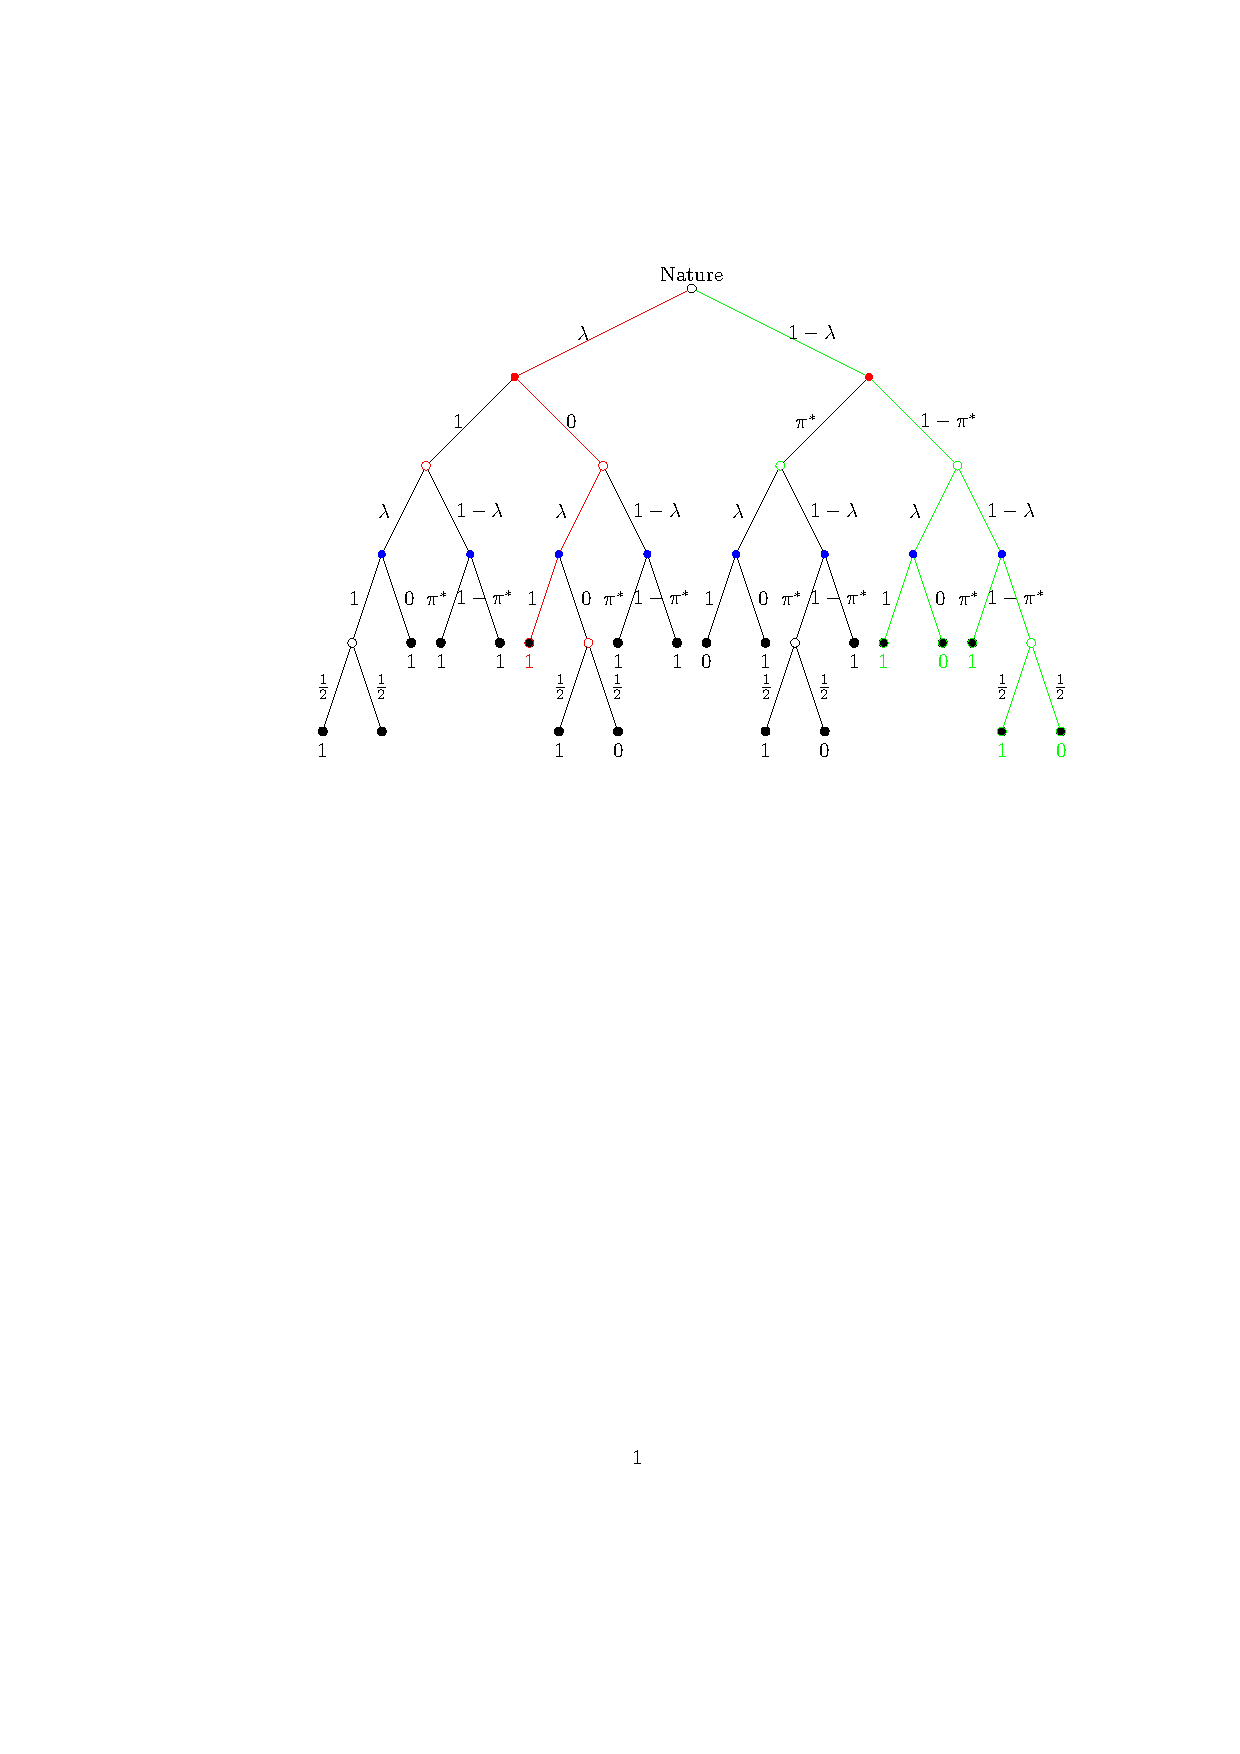
\includegraphics{tikz_example}
\par\end{center}

From an outsider's perspective there are many things happening in
this model. First, one might say that nature determines whether each
of the workers is high or low. In the figure above, the nodes that
represent this are the open nodes. For example, at the very top of
the tree there is an open node that represents nature choosing whether
worker 1 will be a high type, which occurs with probability $\lambda$,
or a low type, $1-\lambda$. The two edges or branches that extend
below this node represent these different choices, and represent these
choices, and are labeled with the appropriate probabilities. 

A bit lower down the tree, there are some more open circle where nature
chooses whether worker 2 is high or low, and a couple at the very
bottom where nature decides which of the two workers gets the job
in case they both apply to the same firm. We'll get back to that momentarily.

At the end of the first two edges in the diagram, there are two red
nodes. These are places where worker 1 makes a decision about where
to apply - the edge that leads down to the left of these red nodes
represents a decision to apply at firm 1, while the edge that leads
down to the right means apply at firm 2. These edges are labelled
with the probabilities with which the worker actually makes these
choices. As we calculated above, the high type worker will apply to
firm 1 (the high wage firm) with probability 1. So we labelled the
two edges with a $1$ and a $0$ to indicate that this is what we
believe will happen. 

At the rightmost red node, we are thinking about the worker having
a low type. As we calculated above, the low type worker should apply
to firm 1 with probability $\pi^{\ast}$, so we label the edge leading
down to the left with $\pi^{\ast}$ to indicate this, similarly for
the edge leading to the right.

Then, as we move down the tree, we have four more open nodes, indicating
nature's choice for worker 2's type. Finally, at the blue nodes, worker
2 makes a choice about whether to apply to firm 1 or firm 2.

If you follow the branches down through the tree, you will eventually
end up at the black nodes, called terminal nodes. Each of these represents
a complete history of play. For example, the path colored red has
nature choosing high for worker 1, worker 1 choosing to apply to firm
2, nature making player 2 a high type as well, and worker 2 applying
to firm 1.

At the very bottom of the tree, I labeled each of the terminal nodes
with a $1$ if worker 1 gets the job, and with a $0$ otherwise. Since
this path tells me everything that happened, I could label the terminal
node with anything, for example, the payoffs of both players. Here
we'll focus on a simpler thing and just keep track of whether or not
worker 1 gets the job.

We don't know whether or not the red path will be followed. To find
the probability that this particular history will occur we just multiply
together the probabilities that are listed along the edges that make
up the path. Again, along the red path we would calculate $\lambda*0*\lambda*1$
to be the probability that this path will be followed (this probability
is $0$ here because a high type worker 1 would never apply to firm
2).

An \emph{event }is a collection of paths. For example, the event that
the worker is a low type and applies to firm2 is colored green in
the diagram. To find the probability of an event, you find the probability
of each of the paths in the event, then add them all together. For
example, there is a total of 5 paths in the event where the worker
is low and applies to firm 2. The probabilities of each of the paths,
from left to right, are
\[
\left(1-\lambda\right)*\left(1-\pi^{\ast}\right)*\lambda*1
\]
then
\[
\left(1-\lambda\right)*\left(1-\pi^{\ast}\right)*\lambda*0
\]
then
\[
\left(1-\lambda\right)*\left(1-\pi^{\ast}\right)*\lambda*\pi^{\ast}
\]
then
\[
\left(1-\lambda\right)*\left(1-\pi^{\ast}\right)*\lambda*\left(1-\pi^{\ast}\right)*\frac{1}{2}
\]
then
\[
\left(1-\lambda\right)*\left(1-\pi^{\ast}\right)*\lambda*\left(1-\pi^{\ast}\right)*\frac{1}{2}.
\]
Summing these last five lines gives the probability of the event.

We are almost ready to do some reasoning. We need one last concept
- \emph{Bayes Rule. }I copied the following diagram from oscarbonilla.com:

\begin{center}
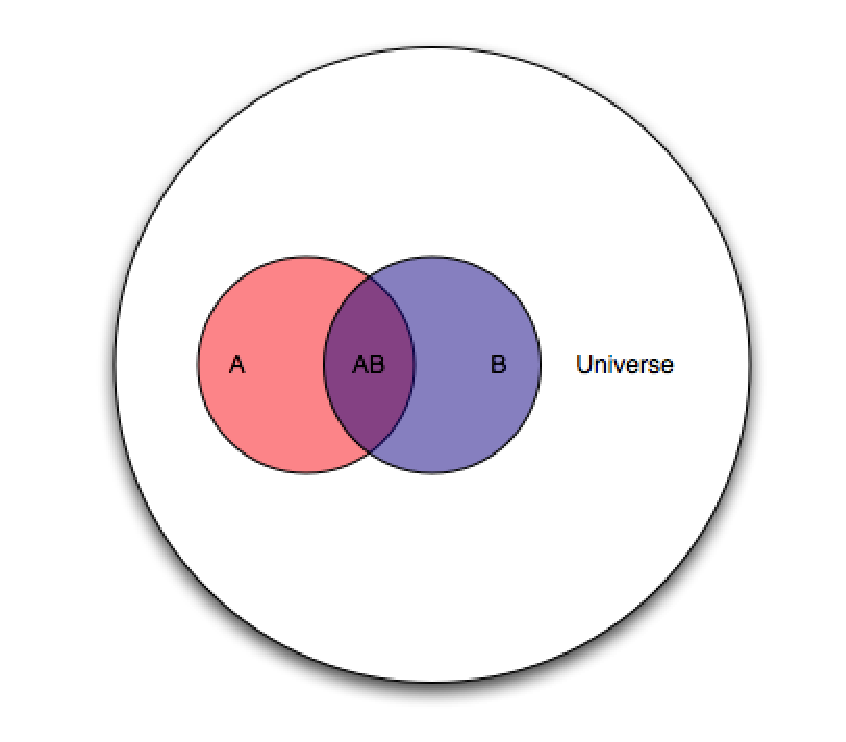
\includegraphics{venn-last}
\par\end{center}

This is the standard way to represent the Bayes rule calculation.
Lets relate it back to the tree diagram that represents our equilibrium.
The big outer (white) circle - labelled Universe - is one way to represent
the collection of all the paths that appear in our diagram. All the
paths together form an event. Since we have to follow one of the paths
in the tree diagram, the event ``something happens'' occurs with
probability 1. In other words, the Universe in the diagram above has
probability 1.

The colored circles in the diagram represent other events. For example,
the circle labelled $A$ in the figure might represent the event in
which the first worker is a high type worker. That event would be
all of the histories that follow the left branch out of the node marked
'Nature' at the very top. You might try to write down the sum of all
the probabilities for those paths as we did above. If you did, you
would find that each string of multiplied probabilities begins with
$\lambda$. If you factored out the $\lambda$, you would have a sum
inside your brackets which would be equal to one (make sure to verify
that for yourself). Then we would say, the probability of the event
in which the first worker is a high type is $\lambda$ and the area
of the colored circle (it looks orange in my browser) marked $A$
in the figure above would be $\lambda$ to represent that.

A second event might be the one where worker 1 finds a job. In the
tree diagram, this is the collection of all the paths that lead to
terminal nodes that have the label $1$ underneath them. Again we
would multiply out the probabilities along each path and sum them
up. The total probability we get from that sum could then be represented
by the area of the blue circle labeled B above.

Notice that the circles overlap, but aren't the same. Thats because
there are paths along which even a high type worker \emph{doesn't}
get a job, and paths along which a low type worker \emph{does }get
a job. Naturally, the area in the intersection of the two circles
represents the event in which worker 1 is both a high type worker,
and that he does get a job. We'd find that probability by collecting
all the paths that start out down the leftward edge at the very top
and also end at a terminal node that has a $1$ beneath it.

If for some reason, someone told us that worker 1 was a high type
worker, we might want to know what the probability is that worker
1 will get a job conditional on this information that he has a high
type. From the diagram, it seems that we could find this by dividing
the area in the intersection of the circles A and B (where he is both
a high type \emph{and }gets a job) by the area of the circle A where
he is a high type. Since you now know it is a mechanical exercise
to compute these areas since they are probabilities derived from the
tree diagram above, you can readily verify that this conditional probability
is

\begin{equation}
Q^{h}=\frac{\lambda}{2}+\left(1-\lambda\right).\label{probability_high}
\end{equation}
This is what Bayes rule says (memorize it because you will need it
a lot), the probability of any event $B$ (for example, he gets a
job) conditional on an event $A$ (for example, we are told he is
a high type) is
\[
\frac{\Pr\left\{ A\cap B\right\} }{\Pr\left\{ A\right\} }.
\]


On the other hand, you should now be able to verify that the probability
that the low type worker gets a job (that is, the probability of getting
a job conditional on being a low type worker) is
\begin{equation}
Q^{l}=\lambda\left(1-\pi^{\ast}\right)+\left(1-\lambda\right)\left\{ \pi^{\ast}\left(\frac{\pi^{\ast}}{2}+\left(1-\pi^{\ast}\right)\right)+\left(1-\pi^{\ast}\right)\left(\pi^{\ast}+\frac{\left(1-\pi^{\ast}\right)}{2}\right)\right\} \label{probability_low}
\end{equation}
Notice that the term multiplying $\left(1-\lambda\right)$ in this
expression must be less than 1. Certainly the low type worker will
do worse than the high type worker when the other worker has a low
type. If the other worker has a high type, the low type worker won't
stand a chance if he or she also applies to the high wage firm. Yet
they don't apply to the high type firm with probability 1. Provided
that $\pi^{\ast}$ close enough to $\frac{1}{2}$, this means that
the probability with which the low type worker matches is smaller
than that for a high type worker. We'll just take this for granted
and leave it for an exercise to figure out when the epxression in
(\ref{probability_low}) will be smaller than the expression in (\ref{probability_high}).
This seems reasonable since the low type worker faces competition
that the high type worker doesn't. The low type worker also uses a
'riskier' application strategy since they deliberately try to compete
against the high type worker where their odds of getting a job are
low.

With this bit of preparation, we can now do some calculations that
will illustrate the usefulness of the new model. We mentioned that
one empirical regularity that seemed inconsistent with our first model
is that the longer a worker remains unemployed, the longer his or
her subsequent unemployment spell is likely to be, and the lower the
wage they get when they finally become re-employed. These facts were
inconsistent with the directed search model we started out with.

The difference now is that we have some unemployment history we can
use to help us make predictions. To do this we need conditional probability
calculations - in particular, one of the things we would like to know
is whether someone who has been unemployed for a period is more or
less likely to get a job than someone who is newly unemployed. 

To do this, lets use the rules above to calculate the probability
that a worker is a high type \emph{conditional }on them having failed
to find a job. Of course, we have to use Bayes rule to do this. The
two events we are interested in are the event in which the worker
fails to find a job - lets call this one event $A$ and the event
that the worker is a high type, call this event $B$. We can now use
the diagram above to see that we need to divide the probability that
the worker is a high type \emph{and }fails to find a job by the probability
that the worker fails to find a job.

If you refer back to our tree diagram, the event where the worker
is a high type is all the paths that lead down the leftmost edge at
the top of the diagram. Along those paths, some of them result in
the worker finding a job (the ones that lead to terminal nodes with
$1$ labelled beneath them), while the other paths lead to outcomes
where the worker remains unemployed (the terminal edges with $0$
below them). Now when a worker appears in the unemployment queue,
the worker has a high type with probability $\lambda$ (at least this
is true provided that job separations are independent of type). 

If the worker has been unemployed for a period already, then from
the logic above (Bayes Rule) the probability he or she is a high type
worker is just
\[
\frac{\lambda\left(1-Q^{h}\right)}{\lambda\left(1-Q^{h}\right)+\left(1-\lambda\right)\left(1-Q^{l}\right)}<\lambda
\]
because of the fact that $\left(1-Q^{l}\right)>\left(1-Q^{h}\right).$
So a worker who has been unemployed for a period is less likely to
be a high type worker than is a worker who has just entered the queue
of unemployed workers.

Some more straightforward Bayes Rule calculations provide additional
insight. Suppose that at the end of a period, we see a worker employed
at the high wage, and another worker employed at the low wage. At
the end of the same period, a shock occurs and both workers are laid
off after working for a single period. What wage do we expect each
of the workers to get at their next job? 

We can leave the calculations to an exercise. However, in the equilibrium
we are using to guide our thinking about this, high wage workers don't
apply at low wage firms. So the worker at the low wage job must be
a low type. On the other hand, low type workers do apply for and get
jobs at the high wage. So inuititvely, the worker who was employed
at the high wage is more likely to be a high type worker - though
this isn't guaranteed. So we might expect the worker at the high wage
firm to get a job more quickly (at least whenever $Q_{h}>Q_{l})$
and end up with a higher wage.


\subsection*{Problems:}
\begin{enumerate}
\item Find the equilibrium in the problem above when $y_{1}=y_{2}$. How
does it compare to the model presented in the first section above.
\item What is the symmetric application strategy that maximizes the expected
number or matches? the expected revenue for both firms?
\item Suppose that $\lambda\frac{w_{1}}{2}+\left(1-\lambda\right)w_{1}<w_{2}$.
Write down the conditions that describe the Nash equilibrium for the
workers' application game. Can you find the two application probabilities?
Numerically?
\item Can you provide conditions under which $Q_{l}<Q_{h}$? As a hint,
note that this will depend on $\lambda$, $w_{1}$ and $w_{2}$. To
make this manageable suppose that $w_{1}=\alpha w_{2}$ and let $w_{2}$
be some constant $w$ so that your answer depends only on $\lambda$
and $\alpha$. Try to draw a diagram with $\alpha$ on one axis and
$\lambda$ on the other, dividing the diagram into regions where $Q_{1}>Q_{2}$
(and remember that there are going to be some regions where the high
type worker won't apply for sure to the high wage firm).
\item In the tree diagram, label all the paths in which the worker gets
a job. Use Bayes Rule to calculate the probability that the worker
has a high type conditional on him finding a job.
\item Use Bayes Rule to find the probabiity that a worker gets a job at
each of the two different wages conditional on the two events finding
a job and being a high type worker, then finding a job and being a
low type worker. Use these conditional probability distributions to
calculate the expected wage of low and high type workers conditional
on finding jobs.
\end{enumerate}
\bibliographystyle{econometrica}
\bibliography{refer}

\end{document}
